\section{Mapas Auto-organizados }

\subsection{Introducción}
Este ejercicio consistió en crear un modelo de mapeo de características
auto-organizadas con el objetivo de clasificar documentos. El mapa
auto-organizado que se utilizo fue una grilla bidimensional de 10 filas y 10
columnas. El objetivo de este ejercicio es el de observar espacialmente en la
grilla las distintas clases de los datos.

Para el entrenamiento se utilizo la siguiente formula para obtener la neurona
ganadora $k^*$:

  \[
  k^* = \argmin_{i,j} \lvert\lvert x-w_{i,j} \rvert\rvert
  \]

La regla de entrenamiento en cada patrón luego de obtener la neurona ganadora
es

\begin{equation}
	\Delta W = \eta_t \cdot h_{k^*}(i,j) \cdot (X^{\mu}-W_{i,j})
\end{equation}

donde h es una función que mapea la distancia entre dos neuronas según la
distribución normal.

\[
	h_{k^*}(i, j) = e^{-\frac{d_{k^*}(i,j)^2}{2}}
\]

con $d_{k^*}(i,j)$ es la típica distancia euclidiana entre los puntos de la
grilla (i,j) y la neurona ganadora $k^*$ escalada por un factor de
$1/\sigma_t$, ie.  $ d_{k^*}(i,j) = \frac{\lvert \lvert (i,j)-k^* \rvert
\rvert}{\sigma_t} $

Las funciones de enfriamiento de $\eta$ y $\sigma$ que se utilizaron en cada
iteración $t$ fueron las siguientes:

\[
  \begin{array}{ccc}
    \eta_t & = & \eta_0 \cdot e^{\frac{-x}{\tau_1}} \\
    \sigma_t & = & \sigma_0 \cdot e^{\frac{-x}{\tau_2}} \\
  \end{array}
\]

Este enfriamiento de las variables $\eta$ y $\sigma$ permiten ir disminuyendo
el nivel de aprendizaje y el área de vecindad respectivamente de cada neurona
para que la red a través del tiempo pueda converger a un estado final estable.

\clearpage
\subsection{Resultados}
\subsubsection{Elección de los parámetros}
\begin{itemize}
	\item $\eta_0$: debe elegirse grande de forma tal que al inicio puedan ser
	realizados cambios bruscos por la red para poder organizarse inicialmente.

	\item $\sigma_0$: Inicialmente tiene que ser grande para que el área de
	vecindad pueda abarcar a todos los nodos con esto alcanzaría
	aproximadamente con el tamaño del diámetro de la grilla

\[
	diam = \sqrt{rows^2+cols^2}
\]
	\item $\tau_1$ y $\tau_2$ deben elegirse de forma tal que al terminar todas
	las iteraciones los valores de $\eta$ y $\sigma$ alcancen una pequeña
	proporción de los $\eta$ y $\sigma$ iniciales.

	La cantidad de iteraciones totales es $epochs \cdot training\_size $.
	Entonces si se quiere al final del entrenamiento que $\eta(t) \in (\eta_{f_l}, \eta_{f_u})$.
	Debe cumplirse que

	\[ \frac{t}{ln(\frac{\eta_0}{\eta_{f_l}})} < \tau_{1} < \frac{t}{ln(\frac{\eta_0}{\eta_{f_u}})} \]

	De igual manera si se quiere que $\sigma(t) \in (\eta_{f_l}, \eta_{f_u})$.
	Debe cumplirse que

	\[ \frac{t}{ln(\frac{\sigma_0}{\sigma_{f_l}})} < \tau_{2} < \frac{t}{ln(\frac{\sigma_0}{\sigma_{f_u}})} \]

	En las experimentaciones con las formulas anteriores se buscó que el $\eta$
	final este entre 0.001 y 0.002 y que el $\sigma$ final termine entre 0.1 y
	0.05.

\end{itemize}

También se decidió experimentar preprocesando la entrada de la red neuronal
para reducir la dimensionalidad de esta.  Para esto se entreno una red tal como
fue explicada en el ejercicio anterior la cual redujo la dimensionalidad
proyectando a 3 componentes principales en algunos casos y 9 en otros.

Por lo anteriormente explicado para el entrenamiento se utilizaron los
siguientes parámetros:
%%%%%%%%%%%%%%%%%%%%%%%%%%%%%%%% AGREGAR PARAMETROS
\begin{center}
  \begin{tabular}{|c|c|c|c|c|c|c|c|c|}
    \hline
    filas & columnas & epochs & $\eta_0$ & $\sigma_0$ & $\tau_1$ & $\tau_2$ & preprocess & componentes \\
    \hline
	10 & 10 & 100 & 0.1 & 16 & 1300 & 1100 & NO & \ \\
    \hline
	10 & 10 & 100 & 0.1 & 16 & 1300 & 1100 & SI & 3 \\
    \hline
	10 & 10 & 100 & 0.1 & 16 & 1300 & 1100 & SI & 9 \\
    \hline
	25 & 25 & 100 & 0.1 & 36 & 1300 & 1100 & NO & \  \\
    \hline
	25 & 25 & 100 & 0.1 & 36 & 1300 & 1100 & SI & 9  \\
    \hline
  25 & 25 & 100 & 0.1 & 36 & 1300 & 1100 & SI & 3  \\
    \hline
  \end{tabular}
\end{center}

Para la visualización de los resultados se realizo un graficó que por cada
muestra del conjunto de entrenamiento con su correspondiente etiqueta, se
calculó cual fue la neurona ganadora. Luego se calculó por cada neurona cual
fue la etiqueta que mas la activó y se la coloreó en base a esa categoría. Cabe
destacar que las neuronas que nunca fueron activadas por ninguna categoría
fueron coloreadas con el color gris.  Los resultados obtenidos fueron los
siguientes

\begin{figure}[H]
  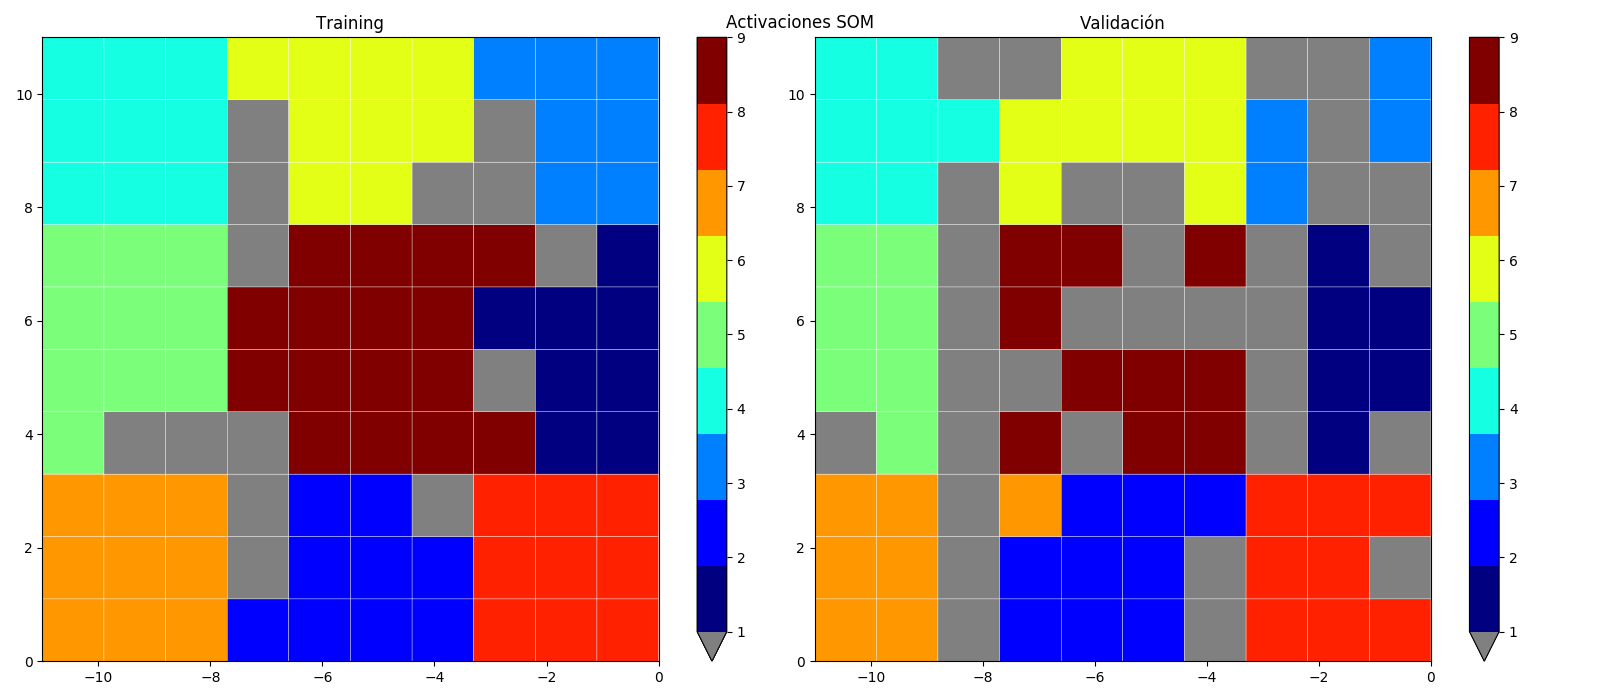
\includegraphics[width=160mm]{imagenes/som_10_10.png}
  \caption{Grilla de 10x10 sin pre-procesamiento}
\end{figure}

\begin{figure}[H]
  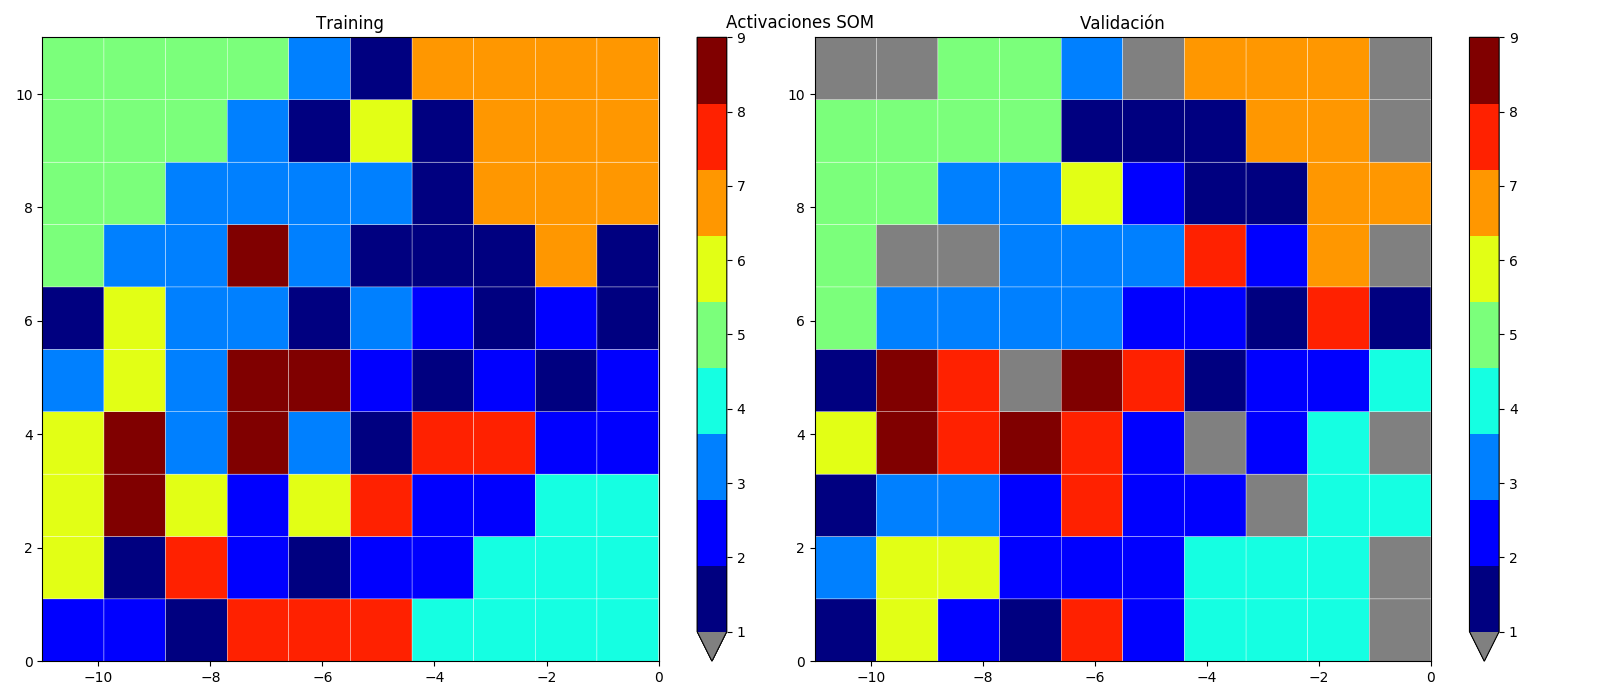
\includegraphics[width=160mm]{imagenes/som_10_10_3_preprocess.png}
  \caption{Grilla de 10x10 con pre-procesamiento y 3 componentes principales}
\end{figure}

\begin{figure}[H]
  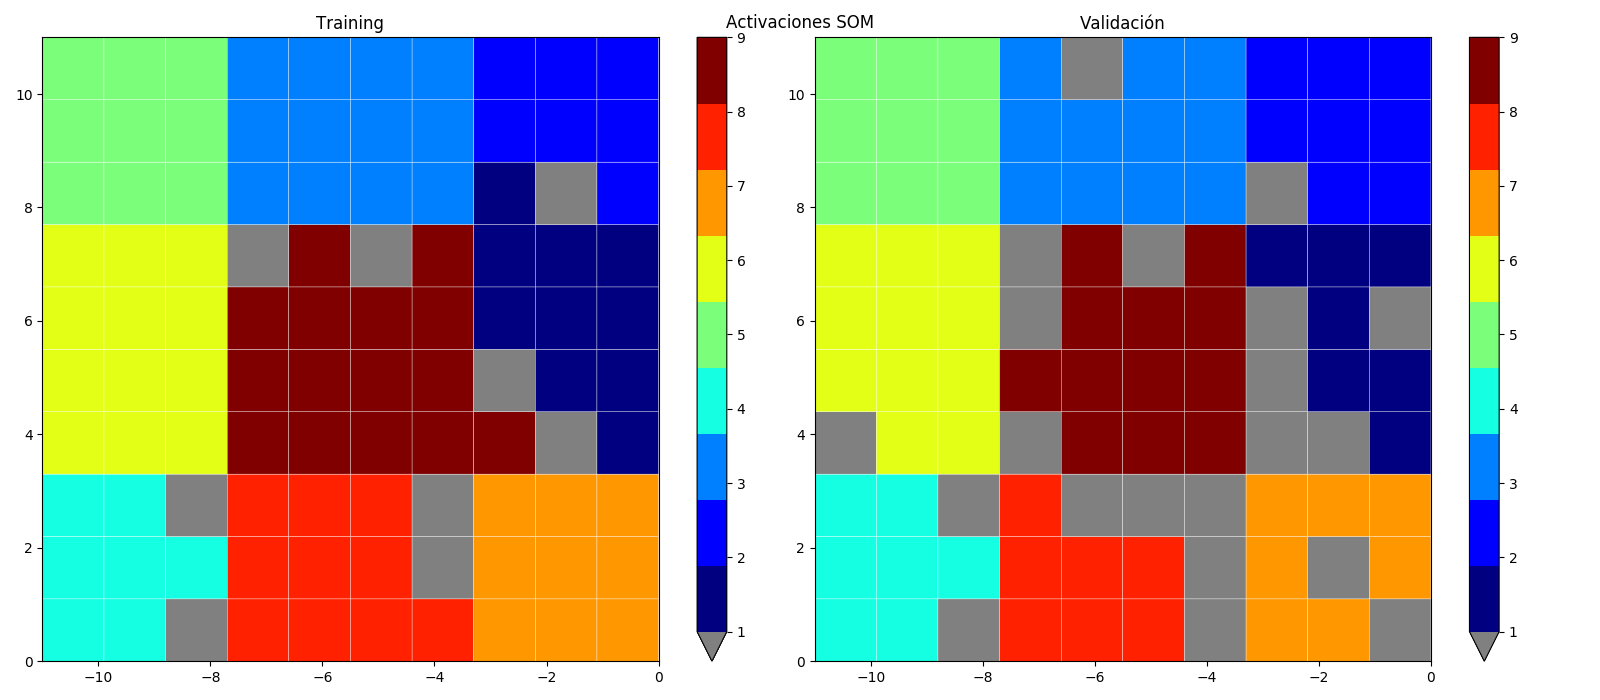
\includegraphics[width=160mm]{imagenes/som_10_10_9_preprocess.png}
  \caption{Grilla de 10x10 con pre-procesamiento y 9 componentes principales}
\end{figure}

\begin{figure}[H]
  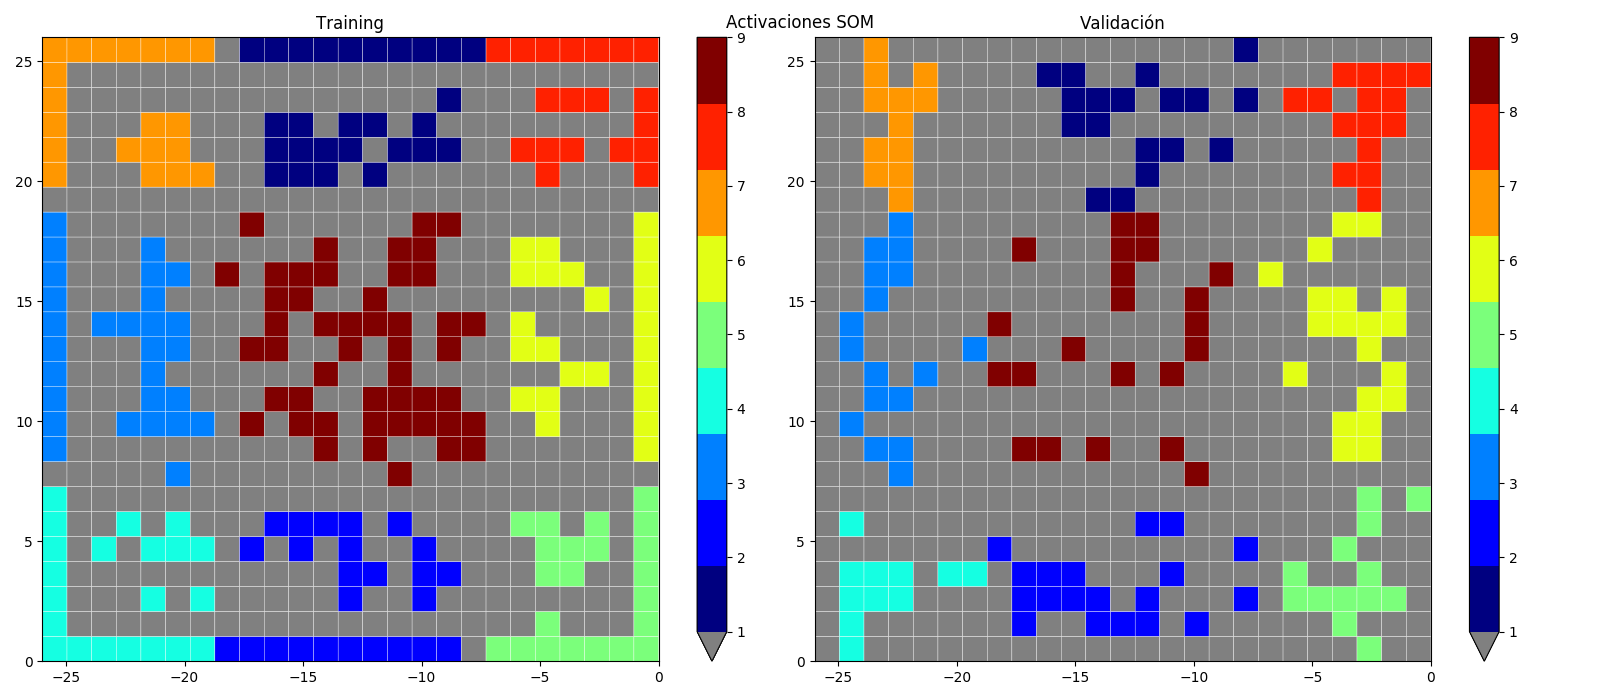
\includegraphics[width=160mm]{imagenes/som_25_25.png}
  \caption{Grilla de 25x25 sin pre-procesamiento}
\end{figure}

\begin{figure}[H]
  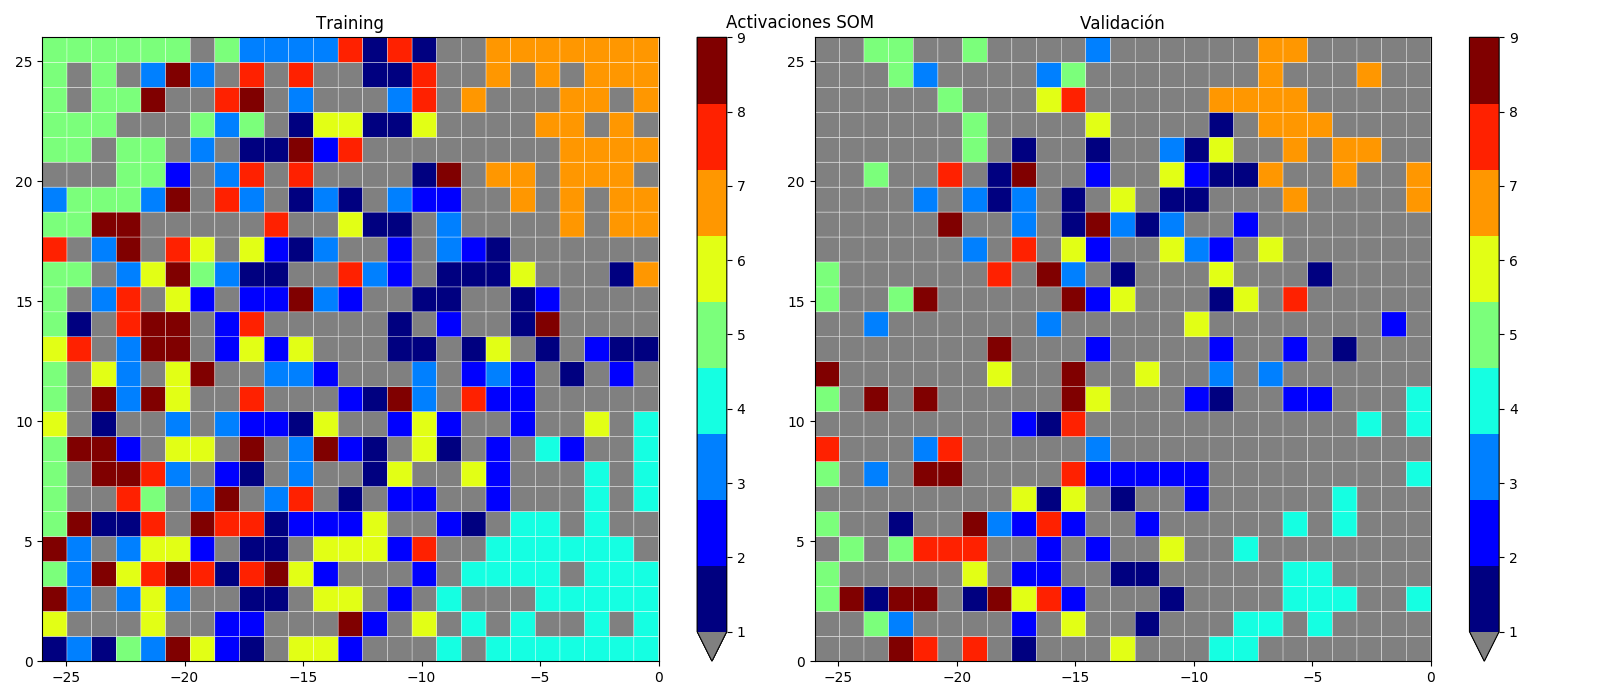
\includegraphics[width=160mm]{imagenes/som_25_25_3_preprocess.png}
  \caption{Grilla de 25x25 con pre-procesamiento y 3 componentes principales}
\end{figure}

\begin{figure}[H]
  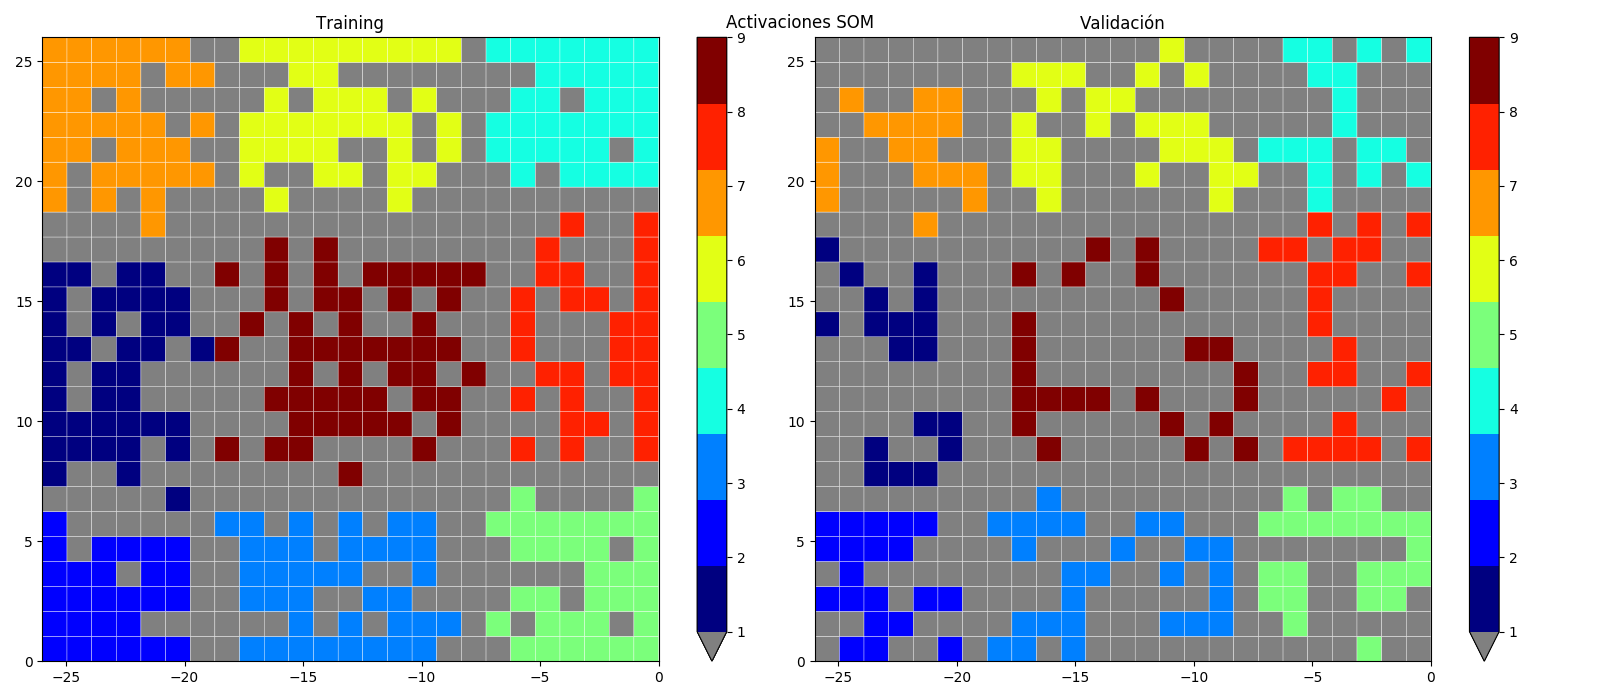
\includegraphics[width=160mm]{imagenes/som_25_25_9_preprocess.png}
  \caption{Grilla de 25x25 con pre-procesamiento y 9 componentes principales}
\end{figure}


\clearpage
\subsection{Conclusión}
Una conclusión que se observo fue la diferencia en los tiempos de entrenamiento
de la red con pre-procesamiento con respecto al entrenamiento sin preprocesado.
Esto tiene sentido ya que se esta entrenando con una entrada de menor
dimensionalidad logrando que el computo realizado sea menor teniendo en cuenta
aun el tiempo de  preprocesado.  Con respecto a la calidad obtenida por cada
experimento se concluyo que la calidad de la red con pre-procesamiento es
superior a la red sin pre-procesamiento, considerando calidad
la forma en la que la red agrupa instancias, es decir la forma de los clusters.

Con respecto a los datos de testeo se observo que el mapa generado presenta una
mayor cantidad de neuronas en color gris, esto quiere decir que hay mas
neuronas que nunca se activan en el testing en comparación con el
entrenamiento.

También se observo que al preprocesar tomando 3 componentes principales se
pudieron distinguir 3 clusters del resto pero sin poder diferenciarse entre si.
El resto de los clusters se entremezclaron con facilidad sin lograr hacer una
distinción. Esto no sucedió cuando se tomaron 9 componentes principales, caso
en el que se lograron visualizar los 9 clusters bien definidos.

Se observo que la red agrupa siempre en 9 clusters similares pero no siempre
los mismos colores se mapean a las misma distribución espacial. Esto no ocurre
con el cluster central que siempre le asigna la categoría 9 (color bordo).
